\documentclass{article}
\usepackage[utf8]{inputenc}
\usepackage[margin=1in]{geometry}
\usepackage[colorlinks]{hyperref}
\usepackage{graphicx}
\usepackage{caption}
\usepackage{color}
\usepackage{subcaption}
\usepackage{float}
\makeatletter
\renewcommand\paragraph{\@startsection{paragraph}{4}{\z@}%
            {-2.5ex\@plus -1ex \@minus -.25ex}%
            {1.25ex \@plus .25ex}%
            {\normalfont\normalsize\bfseries}}
\makeatother
\setcounter{secnumdepth}{4} % how many sectioning levels to assign numbers to
\setcounter{tocdepth}{4}    % how many sectioning levels to show in ToC
\begin{document}
\title{\textbf{CS6011: Kernel Methods for Pattern Analysis}
\\
\textbf{Programming Assignment 3}
}
\author{Aravind Sankar CS11B033 \\
Ramnandan SK CS11B061 \\
Adit Krishnan CS11B063 \\[0.2in]
Group 2
}
\floatplacement{figure}{H}
\maketitle
\tableofcontents 
\newpage
\section{Objective of the assignment}
This assignment consists of 3 parts. 
\begin{itemize}
\item \textbf{Classification} \\[5pt]
Classification using C-SVM with Linear, Polynomial ,Gaussian and Histogram Intersection kernels (for the image data) and $\nu$-SVM with Gaussian kernel for the linearly separable, non linearly separable and overlapping datasets, and also for the image data. \\[10pt]
\item \textbf{Regression} \\[5pt]
Regression using $\epsilon$ and $\nu$-SVR, both using Gaussian kernels, for univariate and bivariate datasets. \\[10pt]
\item \textbf{Novelty Detection}\\[5pt] 
Application of C-SVDD and $\nu$-SVDD for one class in the overlapping dataset and for Multivariate input data. \\[10pt]
\end{itemize}


\section{Classification Tasks}

\section{Regression Tasks}

\subsection{Dataset 1: 1 dimensional curve fitting data}
\begin{center}
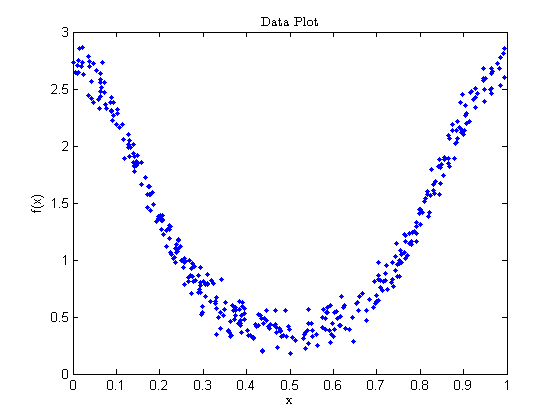
\includegraphics[scale=1]{Regression/univar}
\end{center}
Both $\epsilon$ and $\nu$-SVR with Gaussian Kernels were applied to this dataset.
\subsubsection{$\epsilon$-SVR}
The parameters of interest for $\epsilon$-SVR are $\epsilon$, The value of $\gamma$ in the radial basis function $e^{(-\gamma|u-v|^2)}$ and cost parameter c. They were obtained by narrowing down the ranges (on the log scale) based on experimentation changing one parameter and keeping others fixed, and finally performing cross validation to find the best set of values in the narrowed ranges. \\[5pt]
The best values obtained were $\epsilon$ = 0.0625, c = 4 and $\gamma$ = 16. Following are the corresponding plots.
\begin{center}
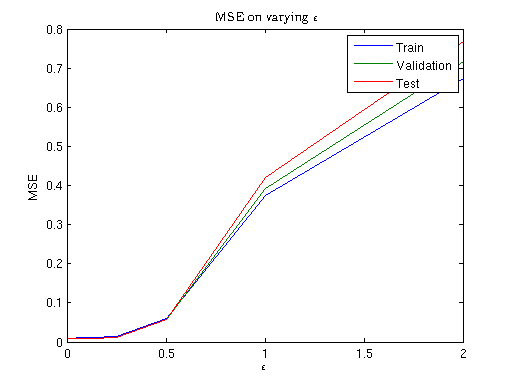
\includegraphics[scale=1]{Regression/mse}
\end{center}
The MSE shows a low value for small values of $\epsilon$ and then goes up for larger values. Having a large value of $\epsilon$ hurts the MSE since we have a wider tube and do not penalize high errors. However the minimum at $\epsilon$ = 0.0625 can be explained as the value for which the tube is sufficiently large to accommodate noise and obtain a good fit, and at the same time not permitting excessive error.
\begin{center}
\includegraphics[scale=1]{Regression/Plot_1}
\end{center}
Clearly, the approximated function is very close to the true function. The next plot shows the variation with the noisy target outputs.
\begin{center}
\includegraphics[scale=1]{Regression/Plot_2}
\end{center}
The plot below shows the Unbounded support vectors (the blue points) which lie on the $\epsilon$ tube and the Bounded ones outside.
\begin{center}
\includegraphics[scale=1]{Regression/Plot_3}
\end{center}
The following are the scatter plots of target and model output. We can see that the model outputs are very close to the targets. 
\begin{center}
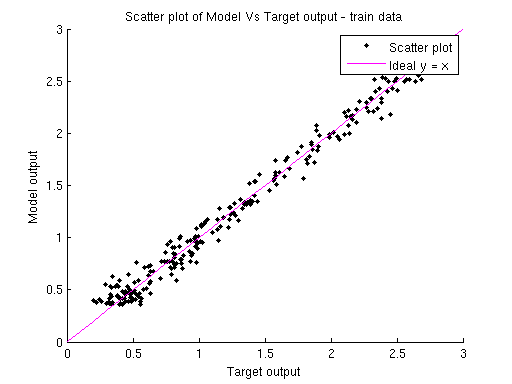
\includegraphics[scale=0.6]{Regression/scatter_train}
\end{center}
\begin{center}
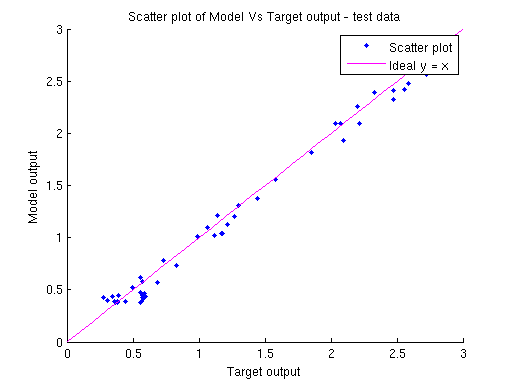
\includegraphics[scale=0.6]{Regression/scatter_test}
\end{center}
\begin{center}
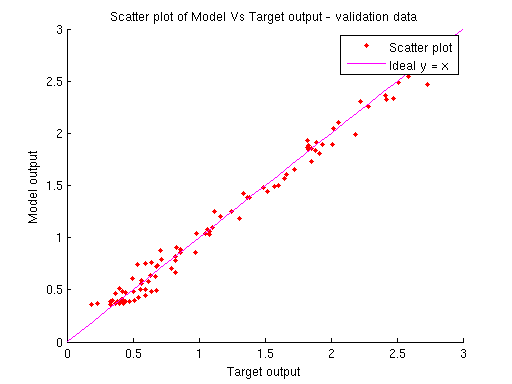
\includegraphics[scale=0.6]{Regression/scatter_val}
\end{center}


\subsubsection{$\nu$-SVR}
In case of a $\nu$-SVR we need to find the parameters $\nu$, c and $\gamma$, latter two being same as in the previous case. Again parameters were found by cross validation in a manner similar to the previous case. \\[5pt]
The best values obtained were $\nu$ = 0.61, c = 16 and $\gamma$ = 16, and using these, $\epsilon$ obtained = 0.0576 which is similar to the previous best value. The purpose of $\nu$ is to tradeoff model complexity vs $\epsilon$ value. Following are the corresponding plots.
\begin{center}
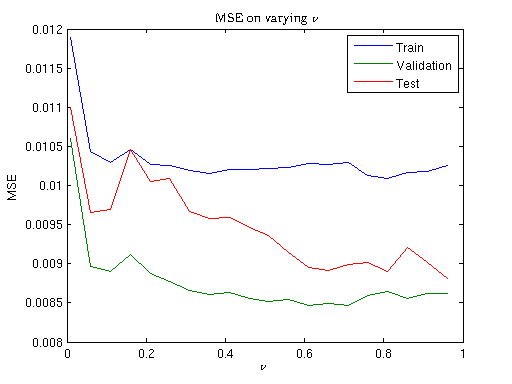
\includegraphics[scale=1]{Regression/nu/mse}
\end{center}
The MSE values here are quite small since the best $\epsilon$ corresponding to each $\nu$ is implicit. A very high value of $\nu$ is restrictive to $\epsilon$, however a very low or 0 $\nu$ allows a choice of relatively large $\epsilon$ without sufficient penalization. Thus both high and very low values of $\nu$ perform poorly.
\begin{center}
\includegraphics[scale=1]{Regression/nu/Plot_1}
\end{center}
Clearly, the approximated function is very close to the true function. The next plot shows the variation with the noisy target outputs.
\begin{center}
\includegraphics[scale=1]{Regression/nu/Plot_2}
\end{center}
The plot below shows the Unbounded support vectors (the blue points) which lie on the $\epsilon$ tube and the Bounded ones outside.
\begin{center}
\includegraphics[scale=1]{Regression/nu/Plot_3}
\end{center}
The following are the scatter plots of target and model output. We can see that the model outputs are very close to the targets. 
\begin{center}
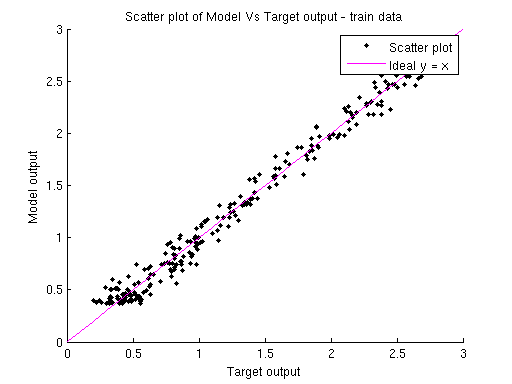
\includegraphics[scale=0.6]{Regression/nu/scatter_train}
\end{center}
\begin{center}
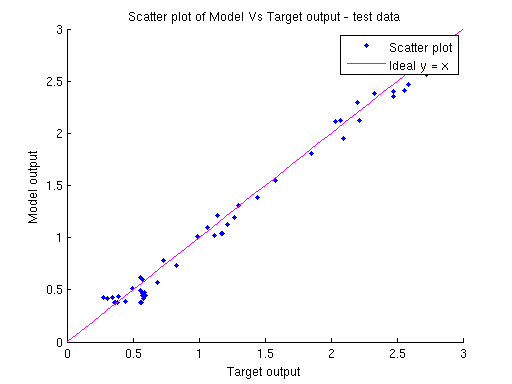
\includegraphics[scale=0.6]{Regression/nu/scatter_test}
\end{center}
\begin{center}
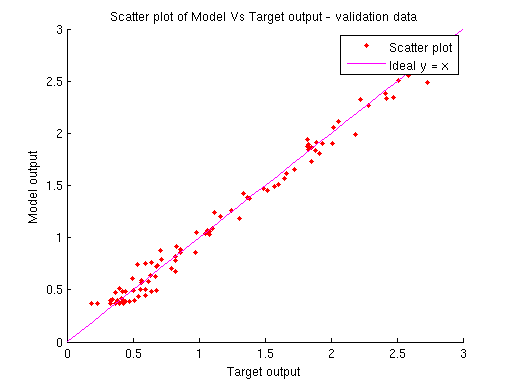
\includegraphics[scale=0.6]{Regression/nu/scatter_val}
\end{center}
Based on the above 2 models, for the univariate data, the performances of the two models are very close and no appreciable difference is seen.
\subsection{Dataset 2: Bivariate data}
\begin{center}
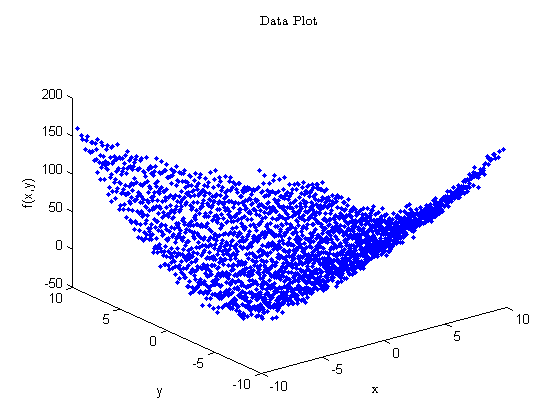
\includegraphics[scale=1]{Regression/bivar/bivar}
\end{center}
Again, we apply $\epsilon$ and $\nu$ SVRs with Gaussian Kernels to this dataset as well.
\subsubsection{$\epsilon$-SVR}
Again. The parameters needed are $\epsilon$, The value of $\gamma$ in the radial basis function $e^{(-\gamma|u-v|^2)}$ and cost parameter c. Similar to the previous case the best values were found using cross validation. The values obtained were c = 512, $\epsilon$ = 2 and $\gamma$ = 0.0039. The values of $\gamma$ is significantly lower than that of the univariate case, This is due to the increased dimensionality of the data. 
\\[5pt]
The cost parameter c is high indicating that deviations ($\zeta$s) are strictly penalized to produce better results. The value of $\epsilon$ is also higher than the univariate case primarily due to the higher dimensionality.
\begin{center}
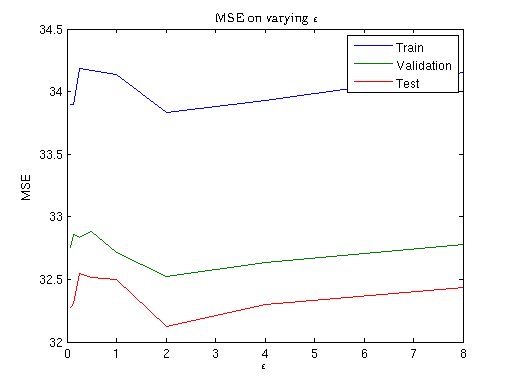
\includegraphics[scale=1]{Regression/bivar/eps/mse}
\end{center}
The minima can be seen at $\epsilon$ = 2 which was the chosen value.
\begin{center}
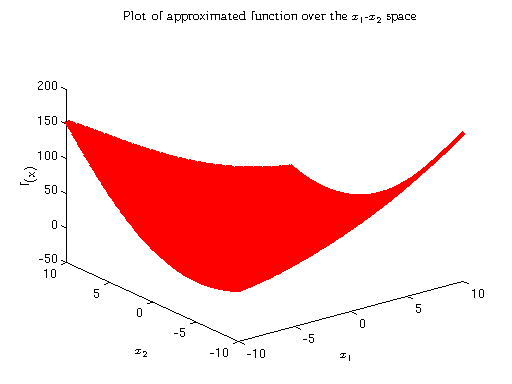
\includegraphics[scale=1]{Regression/bivar/eps/fun}
\end{center}
The above shows the approximated function at the min MSE parameter values.
\\[10pt]
Following are the plots of target and obtained results over the training, test and validation sets.
\begin{center}
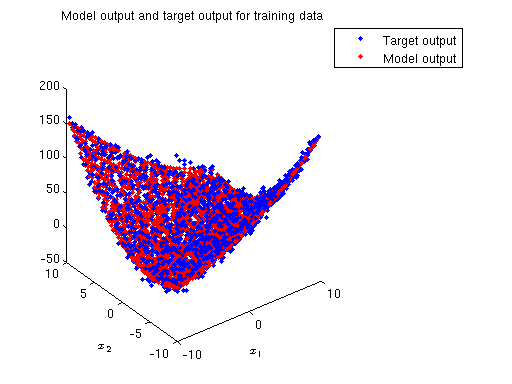
\includegraphics[scale=.6]{Regression/bivar/eps/plot_train}
\end{center}
\begin{center}
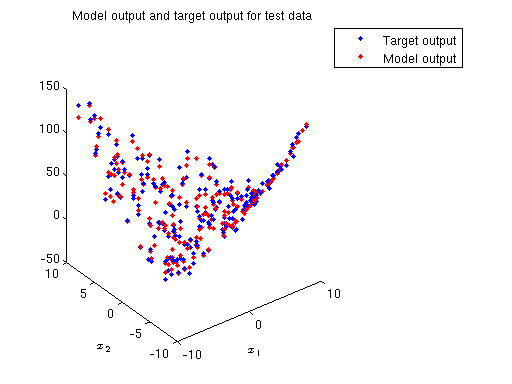
\includegraphics[scale=.6]{Regression/bivar/eps/plot_test}
\end{center}
\begin{center}
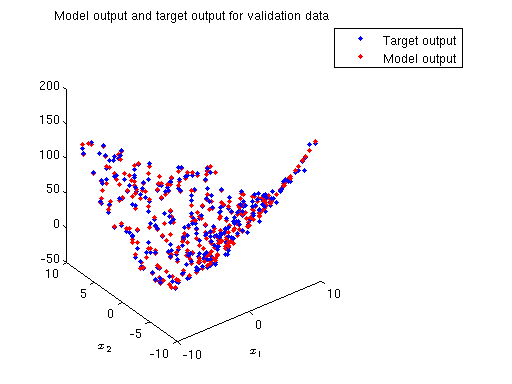
\includegraphics[scale=.6]{Regression/bivar/eps/plot_val}
\end{center}

The scatter plots corresponding to the above results are as follows.
\begin{center}
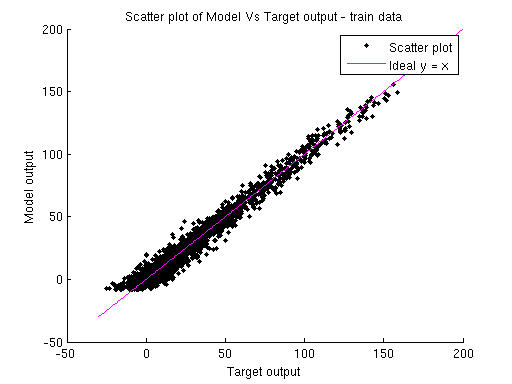
\includegraphics[scale=.6]{Regression/bivar/eps/scatter_train}
\end{center}
\begin{center}
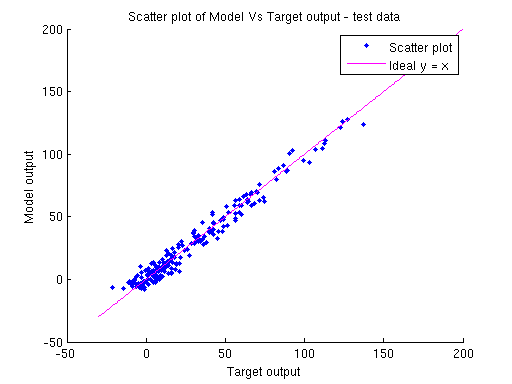
\includegraphics[scale=.6]{Regression/bivar/eps/scatter_test}
\end{center}
\begin{center}
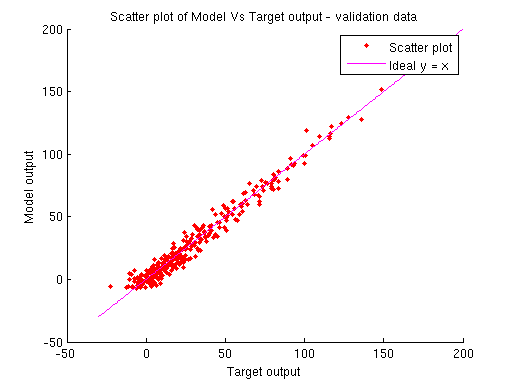
\includegraphics[scale=.6]{Regression/bivar/eps/scatter_val}
\end{center}
\subsubsection{$\nu$-SVR}
In case of $\nu$-SVR applied to this data, the best parameter values obtained were c = 256, g = 0.0039 and nu = 0.61. The corresponding value of $\epsilon$ was 2.897. Following are the plots corresponding to this.
\begin{center}
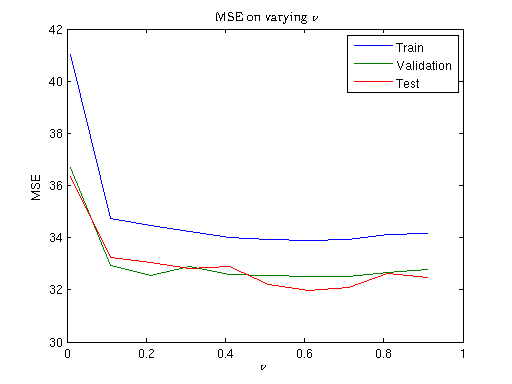
\includegraphics[scale=1]{Regression/bivar/nu/mse}
\end{center}
The minima can be seen at $\nu$ = 0.61 which was the chosen value.
\begin{center}
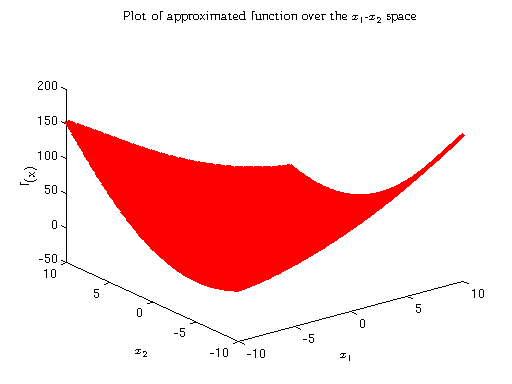
\includegraphics[scale=1]{Regression/bivar/nu/fun}
\end{center}
The above shows the approximated function at the min MSE parameter values.
\\[10pt]
Following are the plots of target and obtained results over the training, test and validation sets.
\begin{center}
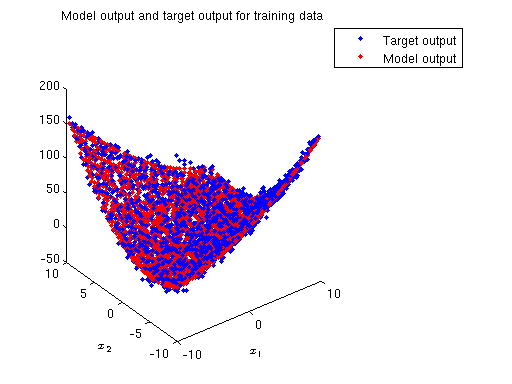
\includegraphics[scale=.6]{Regression/bivar/nu/plot_train}
\end{center}
\begin{center}
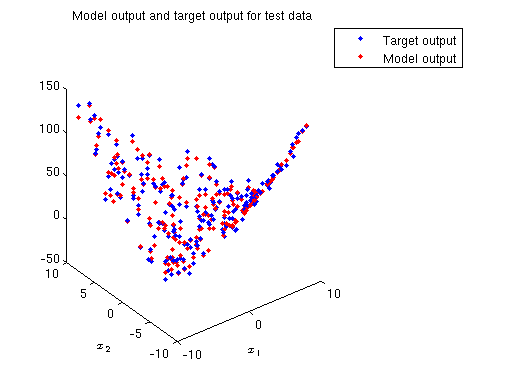
\includegraphics[scale=.6]{Regression/bivar/nu/plot_test}
\end{center}
\begin{center}
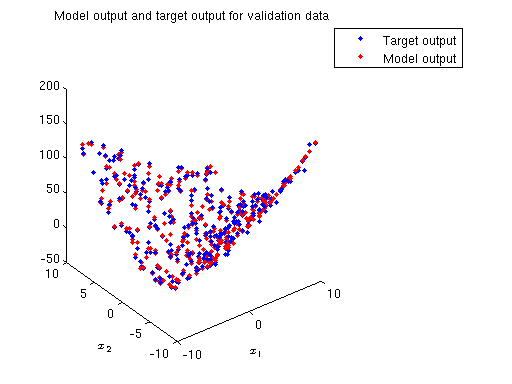
\includegraphics[scale=.6]{Regression/bivar/nu/plot_val}
\end{center}
The scatter plots corresponding to the above results are as follows.
\begin{center}
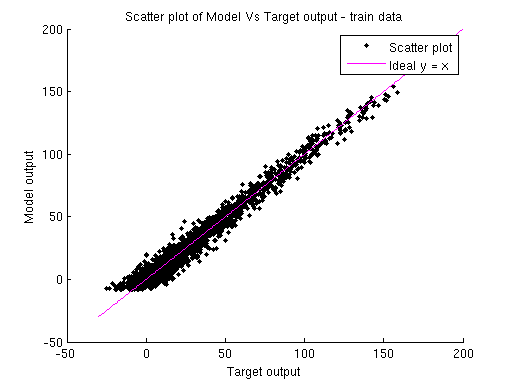
\includegraphics[scale=.6]{Regression/bivar/nu/scatter_train}
\end{center}
\begin{center}
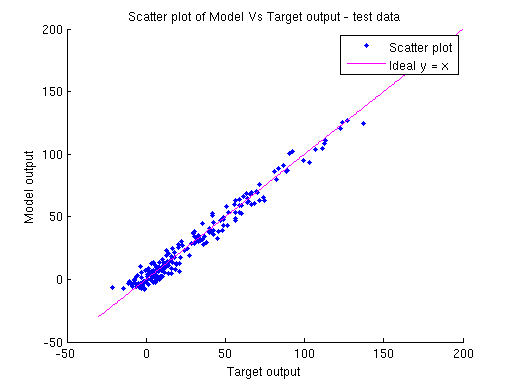
\includegraphics[scale=.6]{Regression/bivar/nu/scatter_test}
\end{center}
\begin{center}
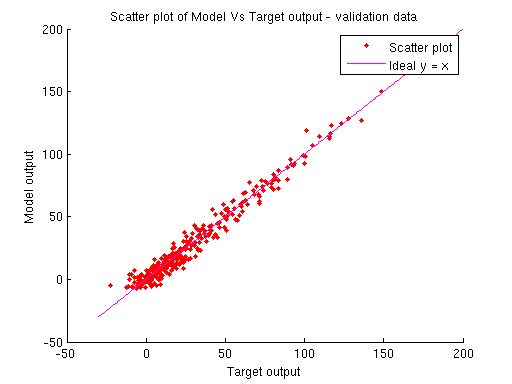
\includegraphics[scale=.6]{Regression/bivar/nu/scatter_val}
\end{center}
\end{document}
